\section{\textit{Noise Generators}}
\label{sec:noise_generators}

El EMS Synthi 100 posee tres generadores de ruido. Este módulo es probablemente el más sencillo de los que podemos considerar <<fuentes>> de sonido. No se encuentra ninguna diferencia en cuanto al diseño de la interfaz entre diferentes versiones del Synthi 100. Está compuesto de dos diales, ambos con los valores entre 0 y 10 (Fig. \ref{fig:noise_generator}):

\begin{description}
	\item[\textit{Colour}] Altera la <<coloración>> del ruido hacia el grave o hacia el agudo. Atendiendo a la descripción de EMS, en su posición central (5), su salida es la de \textit{ruido blanco}, actuando un \textit{filtro pasabajos} cuando se aumenta su valor, y un \textit{filtro pasaaltos} cuando se disminuye.
	\item[\textit{Level}] Nivel de salida.
\end{description}

La implementación de \appName~responde precisamente a esta descripción. Un ruido blanco es filtrado en serie por un \textit{filtro pasaaltos} y un \textit{filtro pasabajos}, cuyas frecuencia de corte entran dentro del espectro audible cuando el valor de \textit{Colour} es respectivamente, mayor o menor que 5.

Este módulo consta de una única salida de audio, ninguna de control de voltaje. No contiene entrada de ningún tipo.

\begin{figure}
	\centering
	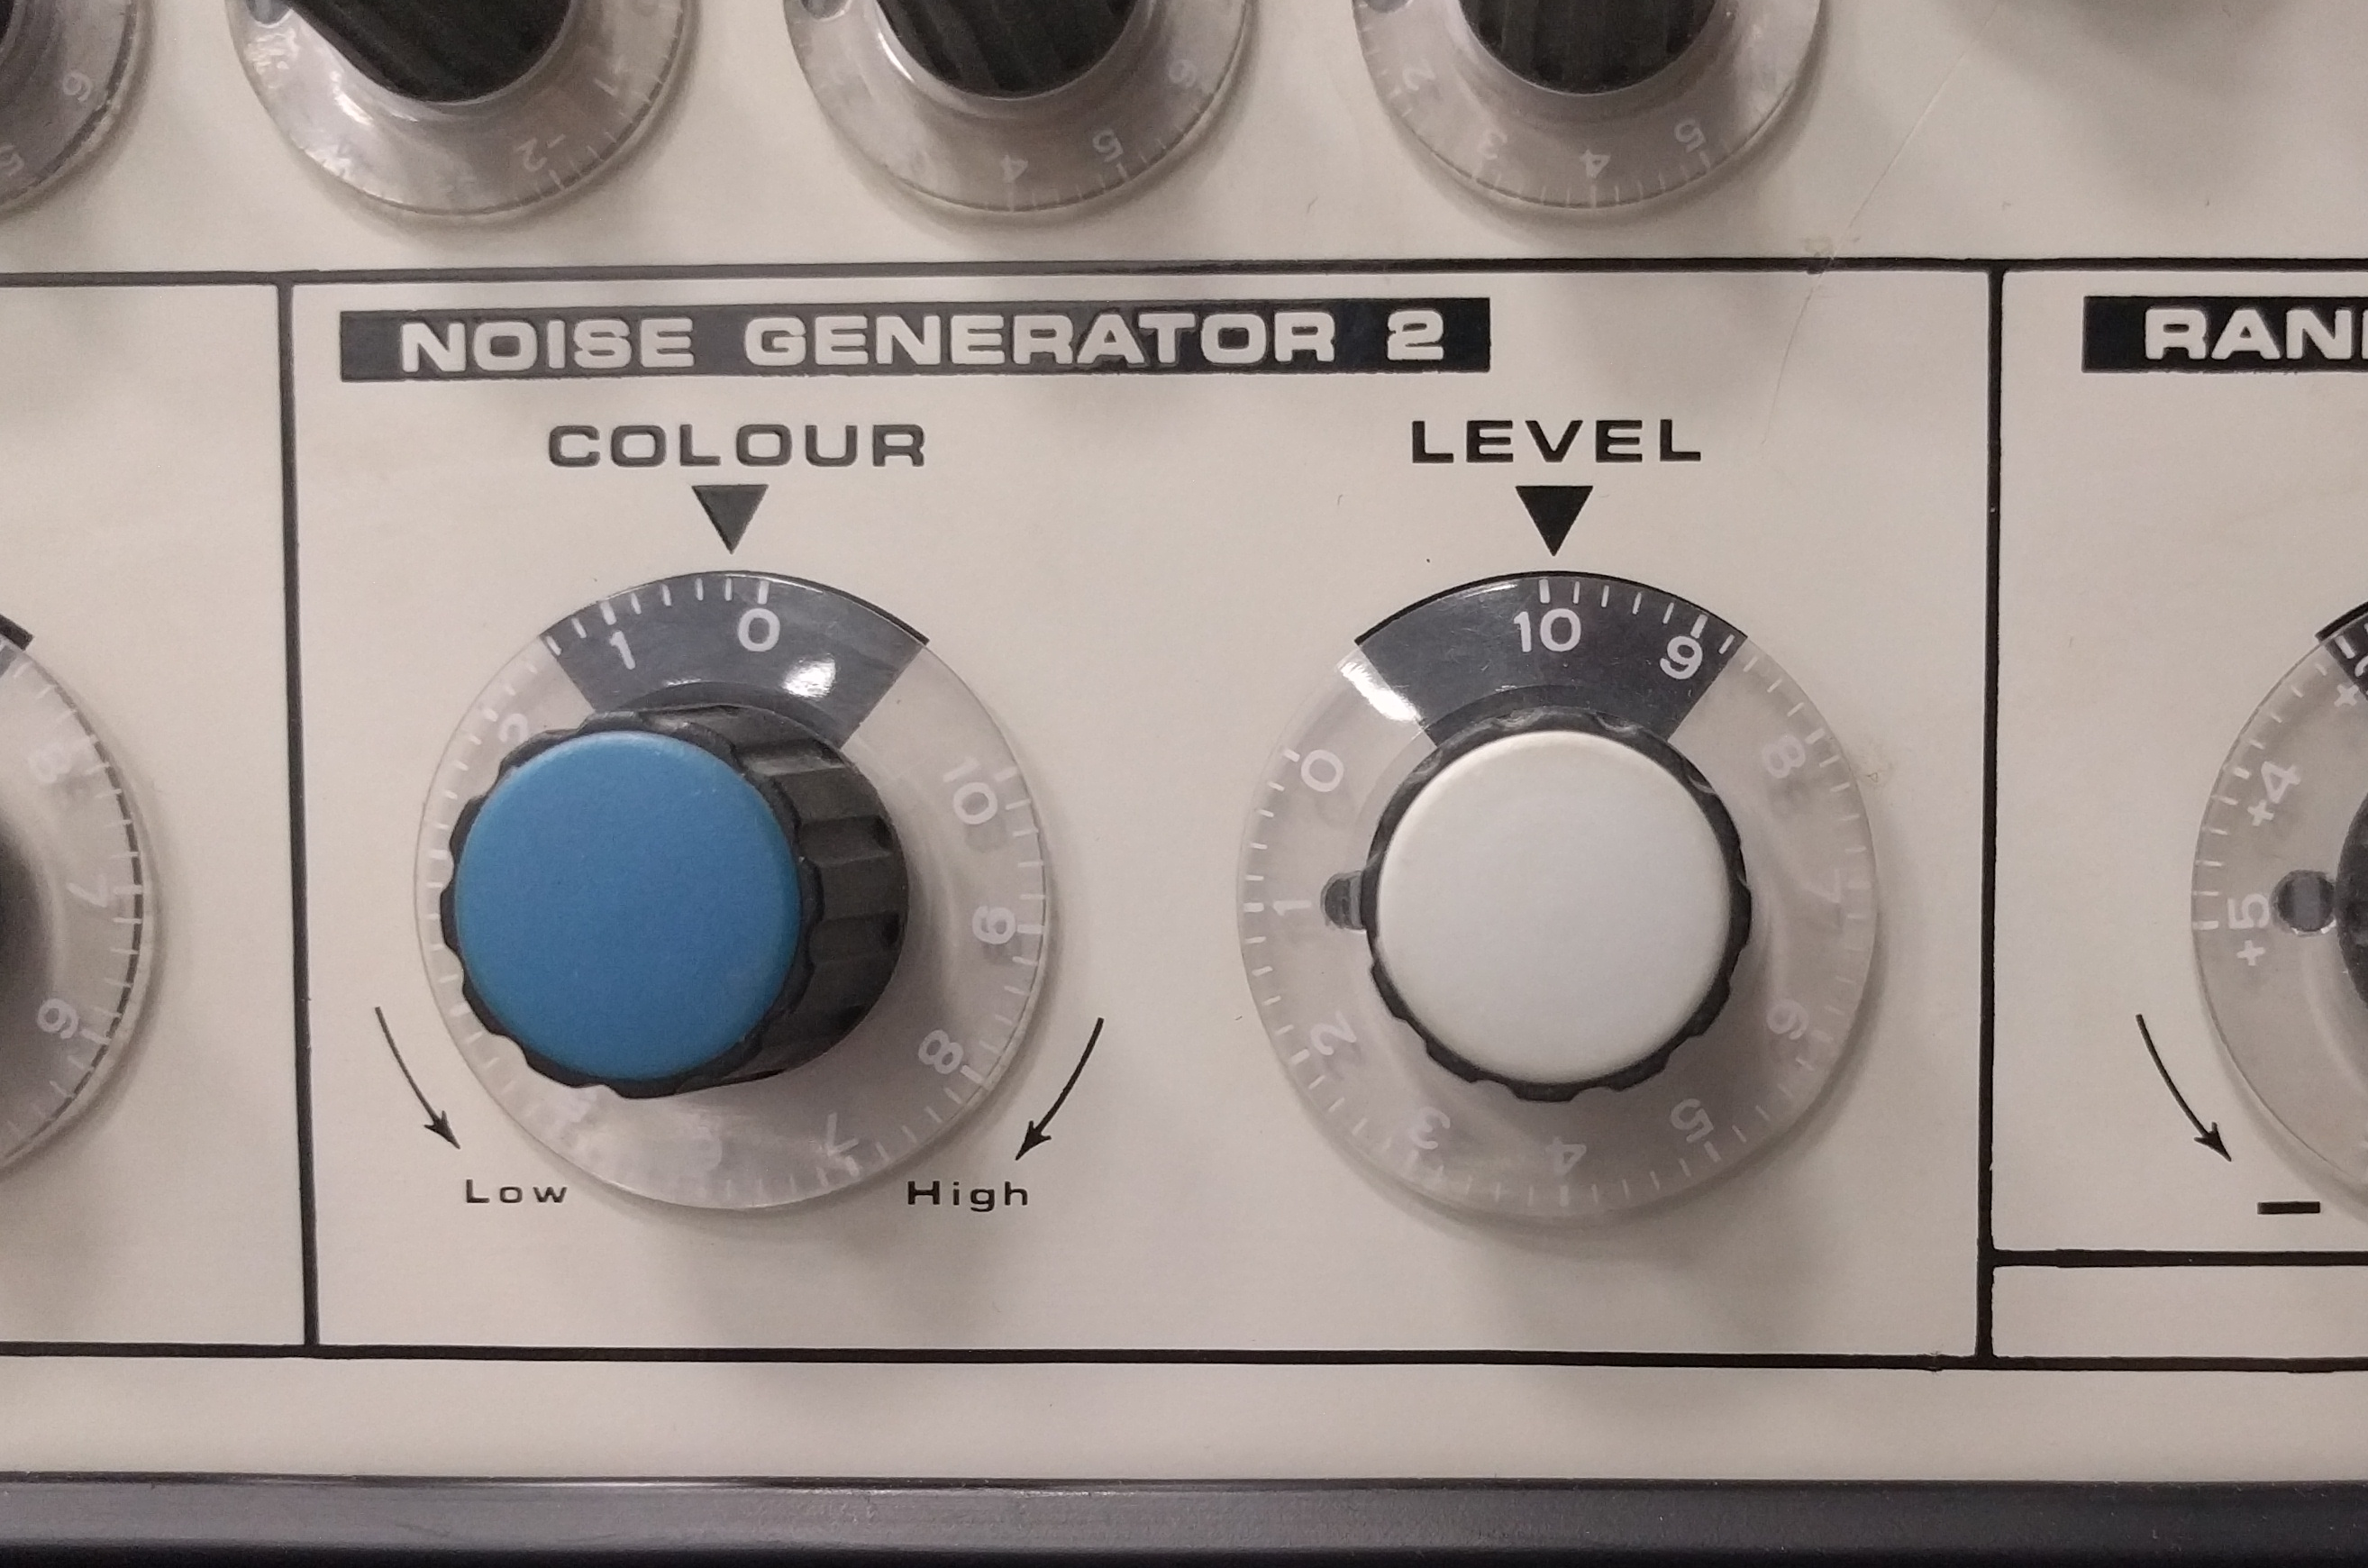
\includegraphics[width=0.7\textwidth]{images/noise_generator}
	\caption{Uno de los dos generadores de ruido del Synthi 100 del GME.}
	\label{fig:noise_generator}
\end{figure}